\section{原子的量子态: 玻尔模型}
\subsection{光电效应}
光电效应中的能量关系: 
\[
\frac{1}{2}mv_m^2=hv-\phi
\]
其中$\frac{1}{2}mv_m^2$为逸出电子的最大动能, $\phi$为逸出功. \textbf{思考}: 当金属带有不同电量时, 上式能否成立, 为什么?

\subsection{玻尔(Bohr)模型}
氢原子中的一个电子绕原子核作圆周运动(经典轨道), 电子只能处于一些分立的轨道上, 它只能在这些轨道上绕核转动, 且不产生电磁辐射. 玻尔模型中的辐射条件:  $h\nu=E_{n'}-E_n$

\subsection{氢光谱}
根据氢原子辐射谱线的巴耳末公式, 里德伯提出了里德伯方程, 氢的所有谱线都可用这个方程表示
\[
\tilde{\nu}=\frac{1}{\lambda}=\frac{1}{B}\Big(\frac{1}{n^2}-\frac{1}{n'^2}\Big),\quad n=3,4,5\cdots,\quad n'=n+1,n+2,n+3\cdots
\]
图\ref{fig03}是氢原子轨道和光谱线示意图.
\begin{figure}[!htb]
\centering
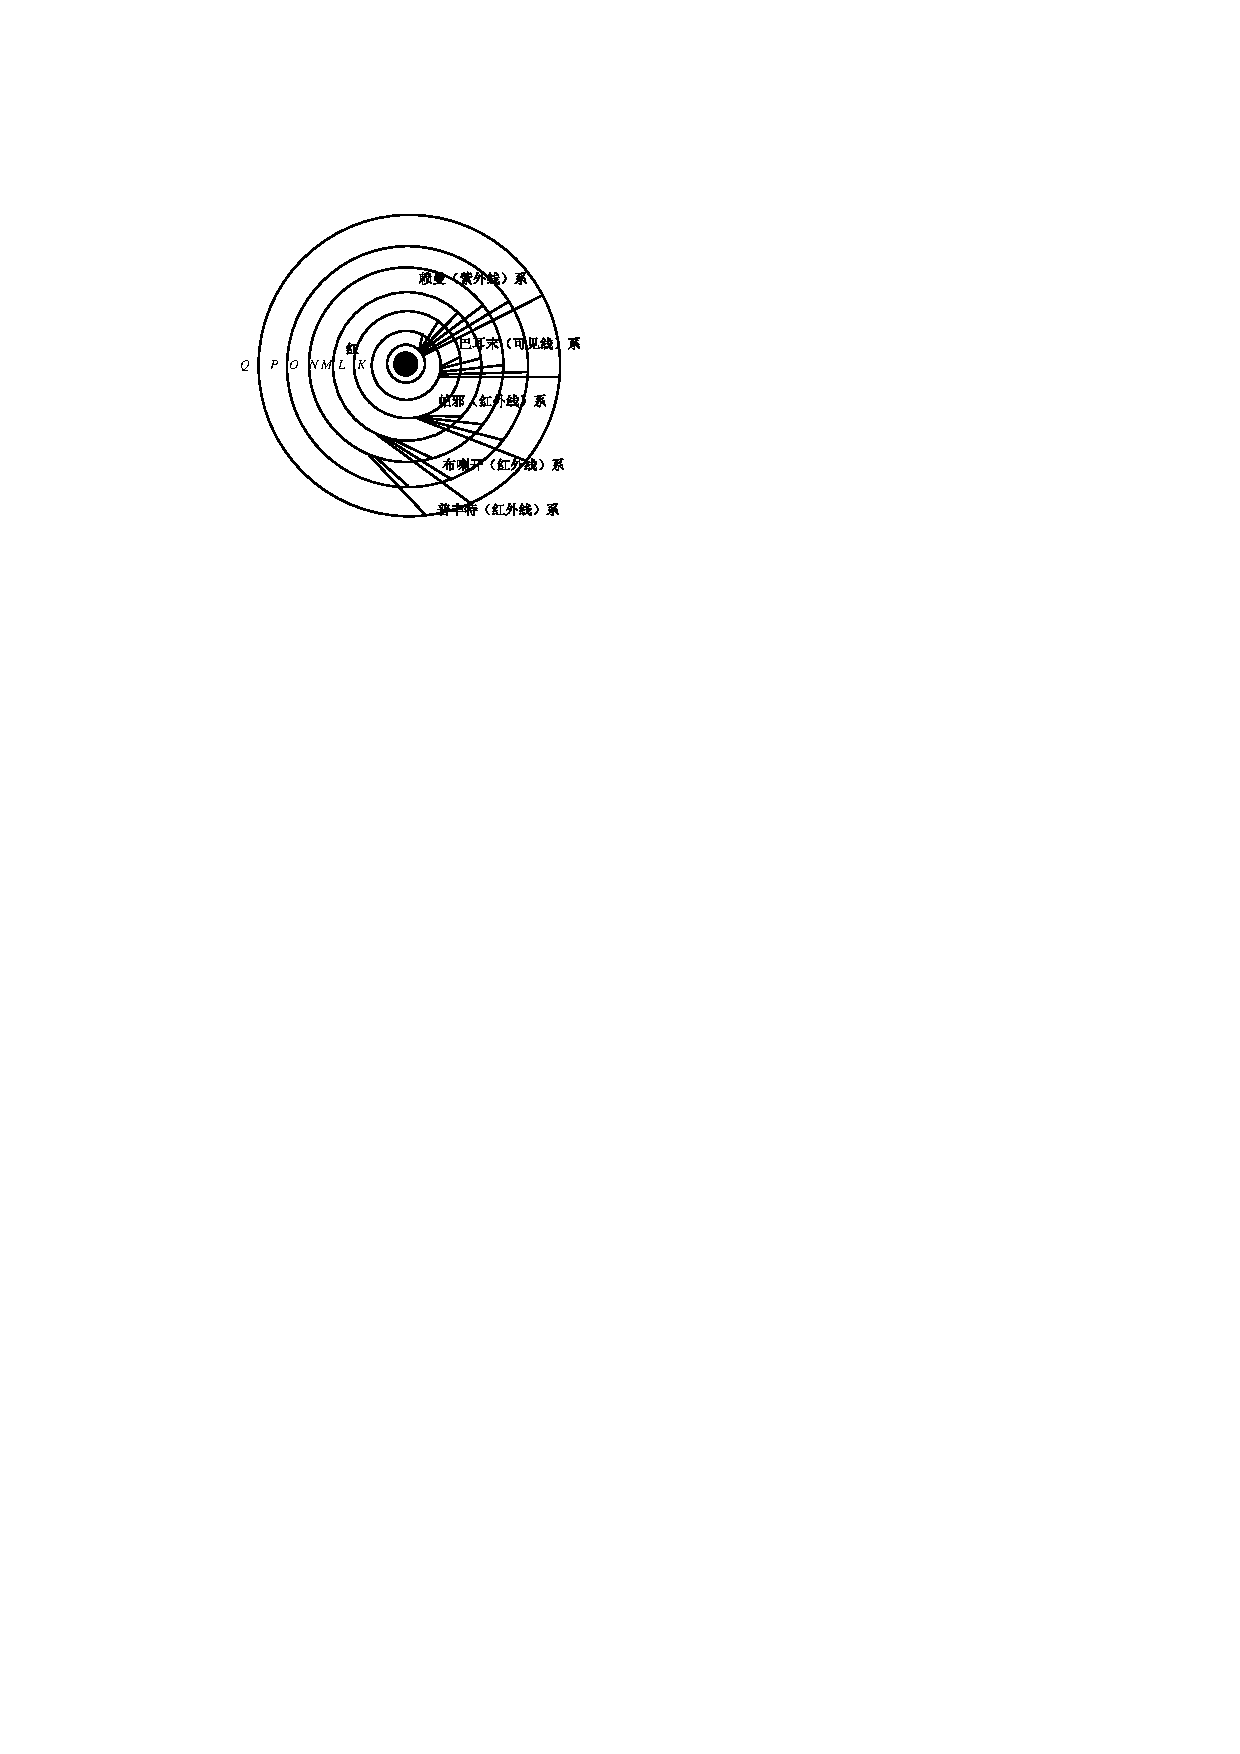
\includegraphics[width=0.3\textwidth]{fig03.pdf}
\caption{\label{fig03}原子轨道和光谱线示意图}
\end{figure}


\subsection{固, 液, 气光谱的成因特点}
\begin{itemize}
\item 固体: 固体光谱是晶格放的光形成的, 但晶格的联系太紧密, 故很少显示出原子状态跃迁发光. 固体光谱为连续谱. 
\item 液体: 液体光谱更多的是分子之间的相互运动, 很少显示出跃迁发光(干扰因素太多). 液体光谱为带状谱. 
\item 气体: 电子跃迁发光. 气体光谱为线状谱. 
\end{itemize}
\noindent[\textbf{思考}]: 要了解原子内部的信息, 为何选用冷光源?

\subsection{夫兰克(Frank)-赫兹(Hertz)实验}

\begin{multicols}{2} 

如右图所示, 电子从热阴极K发出, 经K与G间电场加速. 在G与A之间加反电压, 当电子进入GA空间时, 若有较大能量, 则可以克服反电场到达极A. 若电子在KG区域把能量给了原子, 那么, 电子剩下的能量就不足以克服反电压而抵达A. \textbf{实验表明}: 汞原子对外来能量, 不是``来者皆收'', 而是以4.9eV为单位的吸收能量(气体状态下原子吸收电子的能量是不连续的).
%\begin{figure}[!htb]
%\centering
\begin{center}
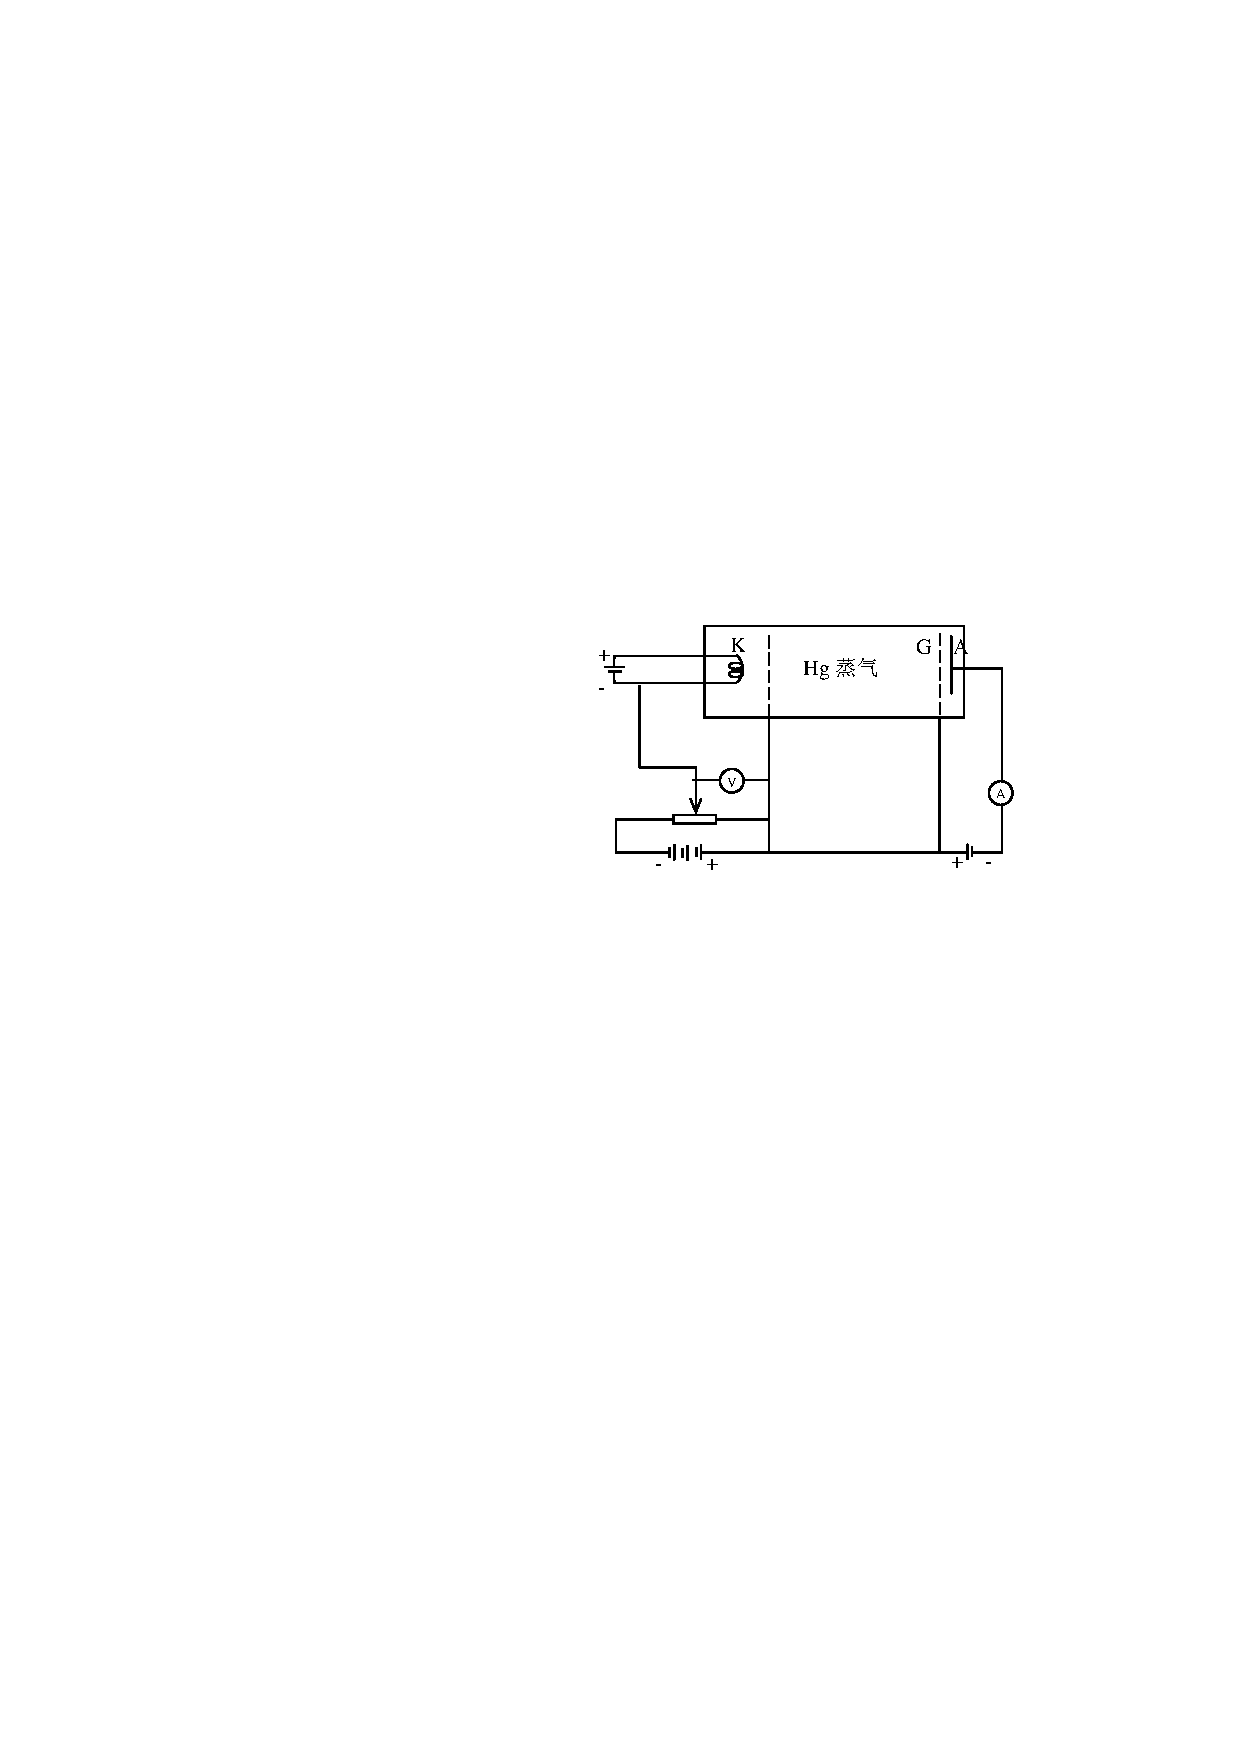
\includegraphics[width=0.3\textwidth]{fig04.pdf}
\end{center}
%\caption{\label{fig04}夫兰克-赫兹实验装置}
%\end{figure}
\end{multicols}

